\section{Methods}
\subsection{Study area}
\label{subsec:studyArea}
I selected for the study system the Drink Planning Area which consists of 7056 ha on the east slopes of the Cascade Mountain Range in the Deschutes National Forest (see Figure \ref{fig:drinkOverview}). This area makes for an adequate study system, because it provides conflicting ecosystem services which the US Forest Service seeks to simultaneously optimize.

\begin{figure}[ht]
\centering
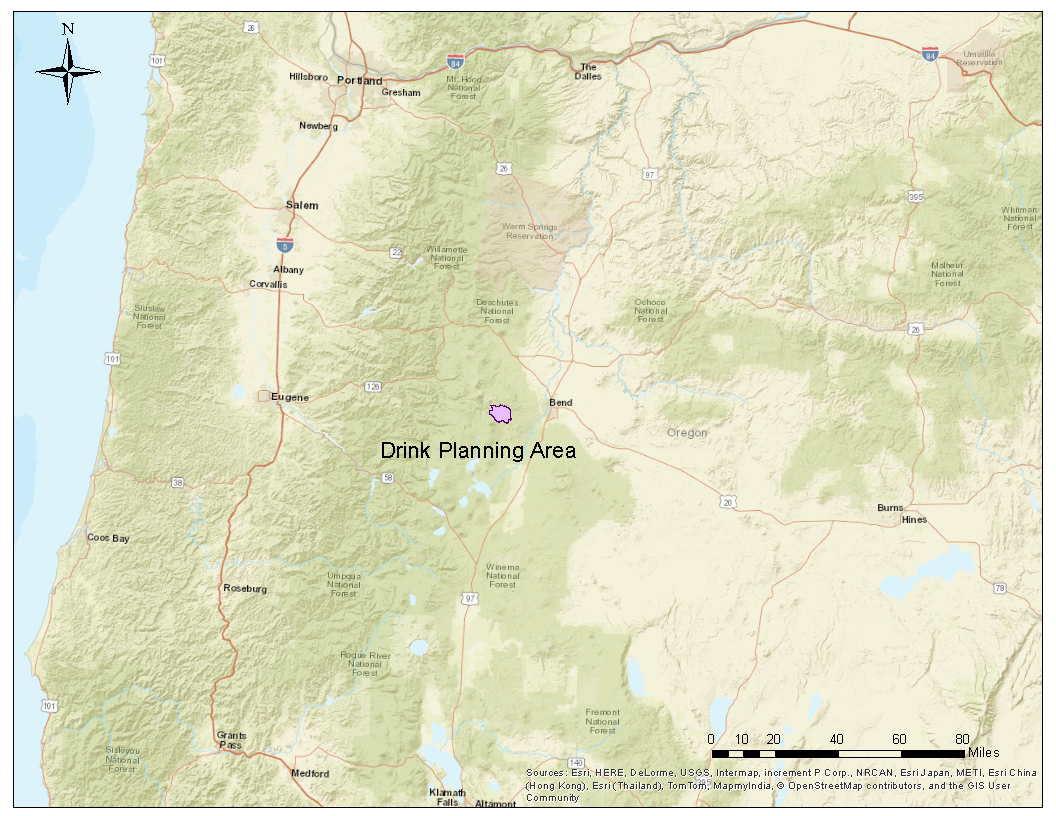
\includegraphics[width=.85\textwidth]{../images/DrinkMap_Overview}
\caption[Overview of the study system, the Drink Planning Area]{Overview of the study system, the Drink Planning Area (in purple), consisting of 7056 ha in the Deschutes National Forest.}
\label{fig:drinkOverview}
\end{figure}

The first objective is the reduction of fire hazard rating through the use of silvicultural treatments. The USFS chose this objective because one third of the Drink area comprises the municipal watershed for the cities of Bend, OR and Sisters, OR (see Figure \ref{fig:drinkOwlAndWatershed}) which have a combined population of approximately 90,000. Wildfires pose a threat to the watershed as they cause soil water repellency, surface runoff, and debris torrents \cite{ice2004effects}.

\begin{figure}
\centering
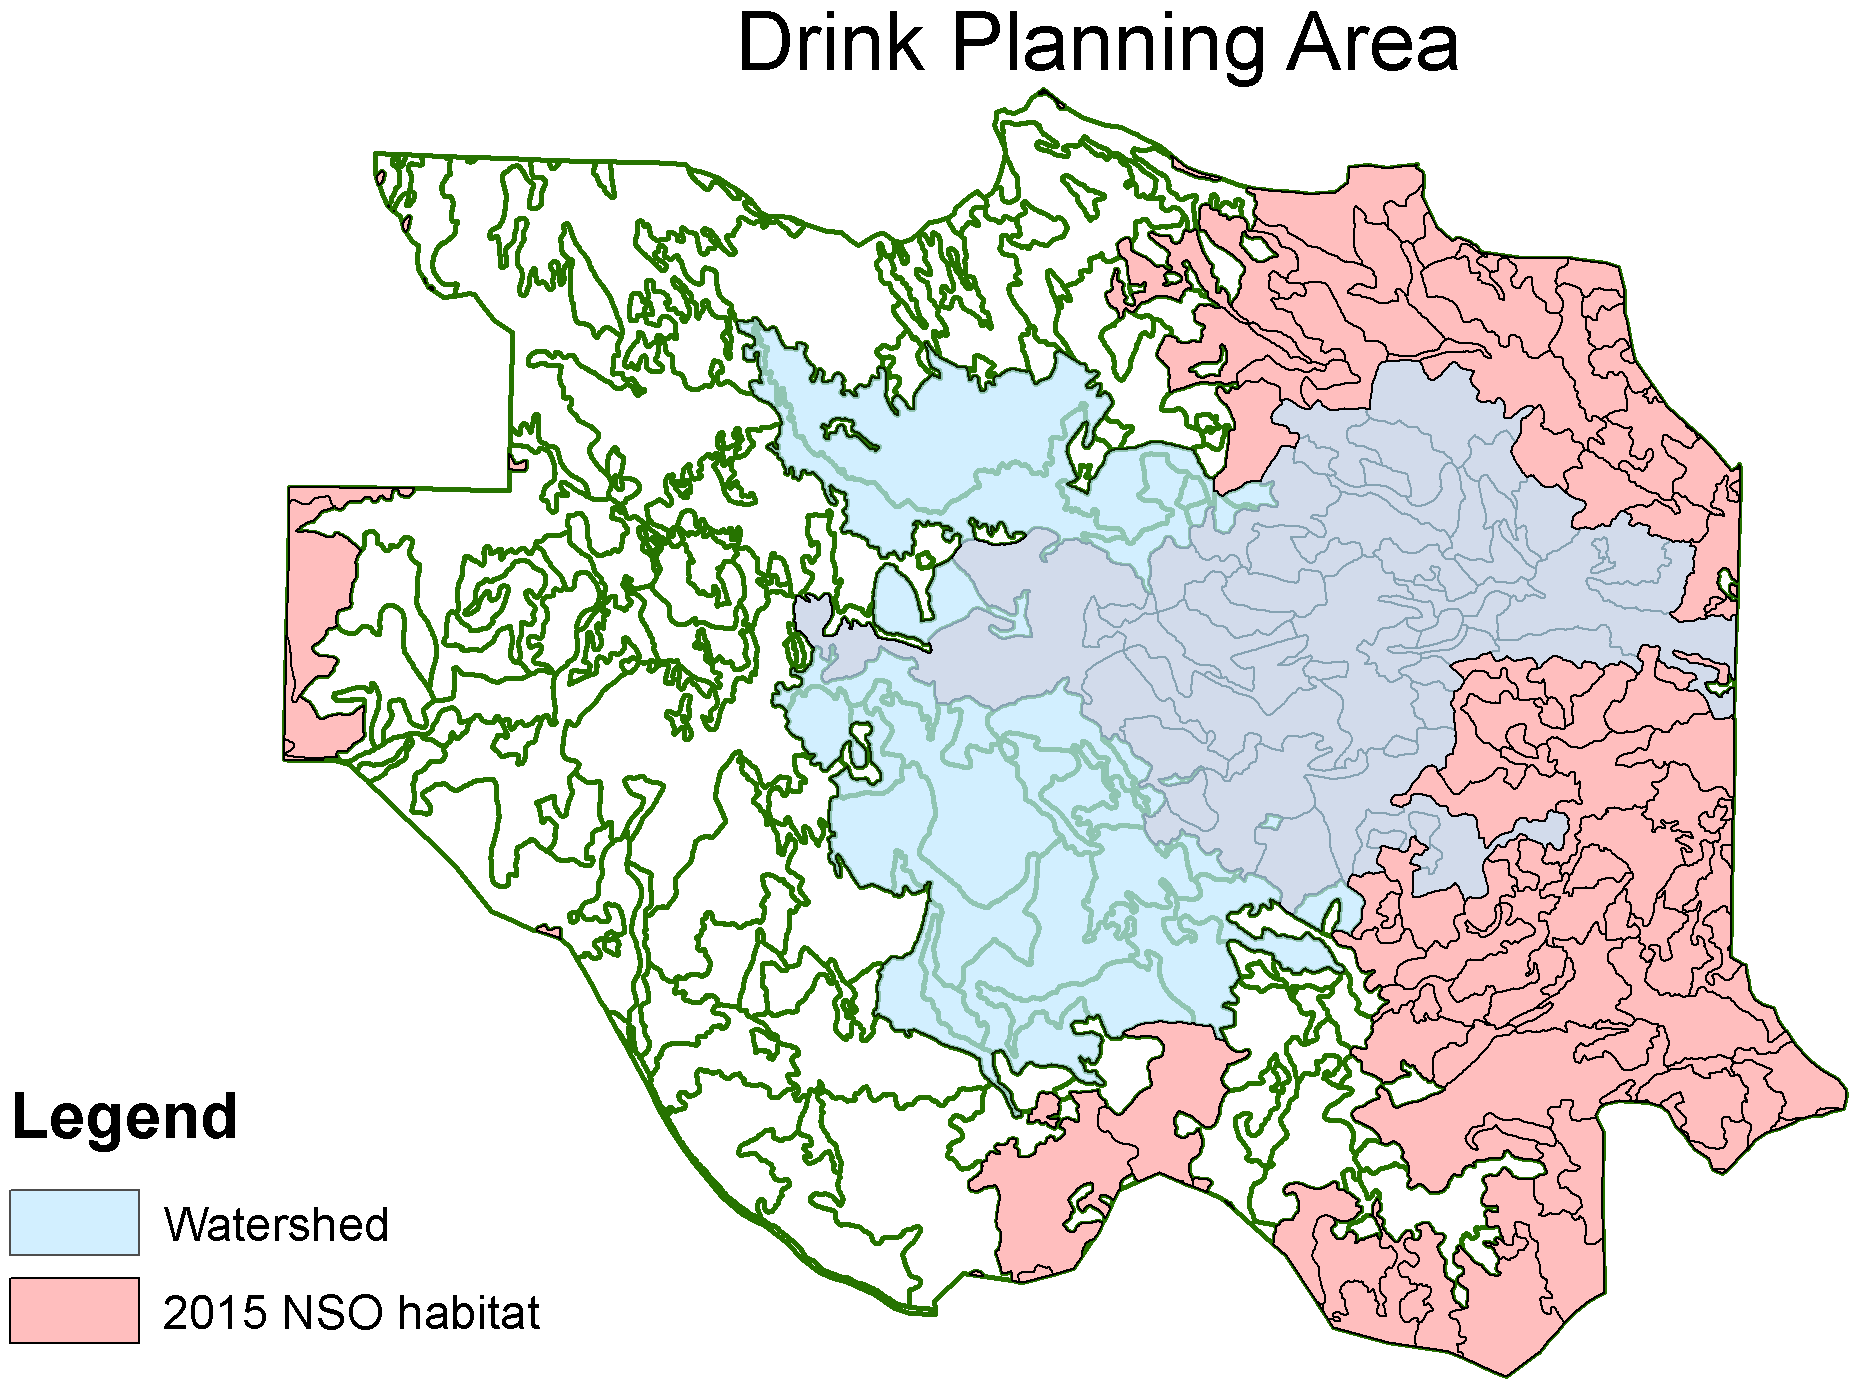
\includegraphics[width=.5\textwidth]{../images/DrinkMap_NSOAndWatershed}
\caption[NSO Habitat and municipal watershed in the Drink Planning Area]{Location of the municipal watershed and the suitable NSO habitat in the Drink area at the beginning of the planning horizon (2015). Interior polygons are the 303 management units.}
\label{fig:drinkOwlAndWatershed}
\end{figure}

In addition, approximately 43\% of the Drink serves as habitat for the northern spotted owl (NSO) (\textit{Strix occidentalis caurina}) (Figure \ref{fig:drinkOwlAndWatershed}). The USFS is required to protect the NSO since it is threatened and therefore protected by the Endangered Species Act of 1973 \cite{congress1973endangered}. The protection of NSO habitat is the second objective considered in this analysis.

Lastly, I aim to minimize the sediment delivered to the watershed as a result of the treatments applied to reduce fire hazard. While the treatments intend to provide long-term protection of the quality of the watershed, they also have the potential to introduce short-term increases in sediment delivery \cite{o2005conceptual}.

To accomplish long-term reduction in fire hazard rating for the area, I formed a strategic plan for silvicultural treatments to apply across the Drink. The treatments may be applied in each of two 20-year time periods (2015-2035 and 2035-2055) and to each of the 303 management units that comprise the Drink. The division of the management units (stands) was performed \textit{a priori} by the Forest Service. The decision as to which treatment to perform on a stand is entirely dependent on silvicultural characteristics; the rules used to determine the treatment applications can be found in Appendix \ref{chap:appBTreatmentSpec}.

\begin{figure}
\centering
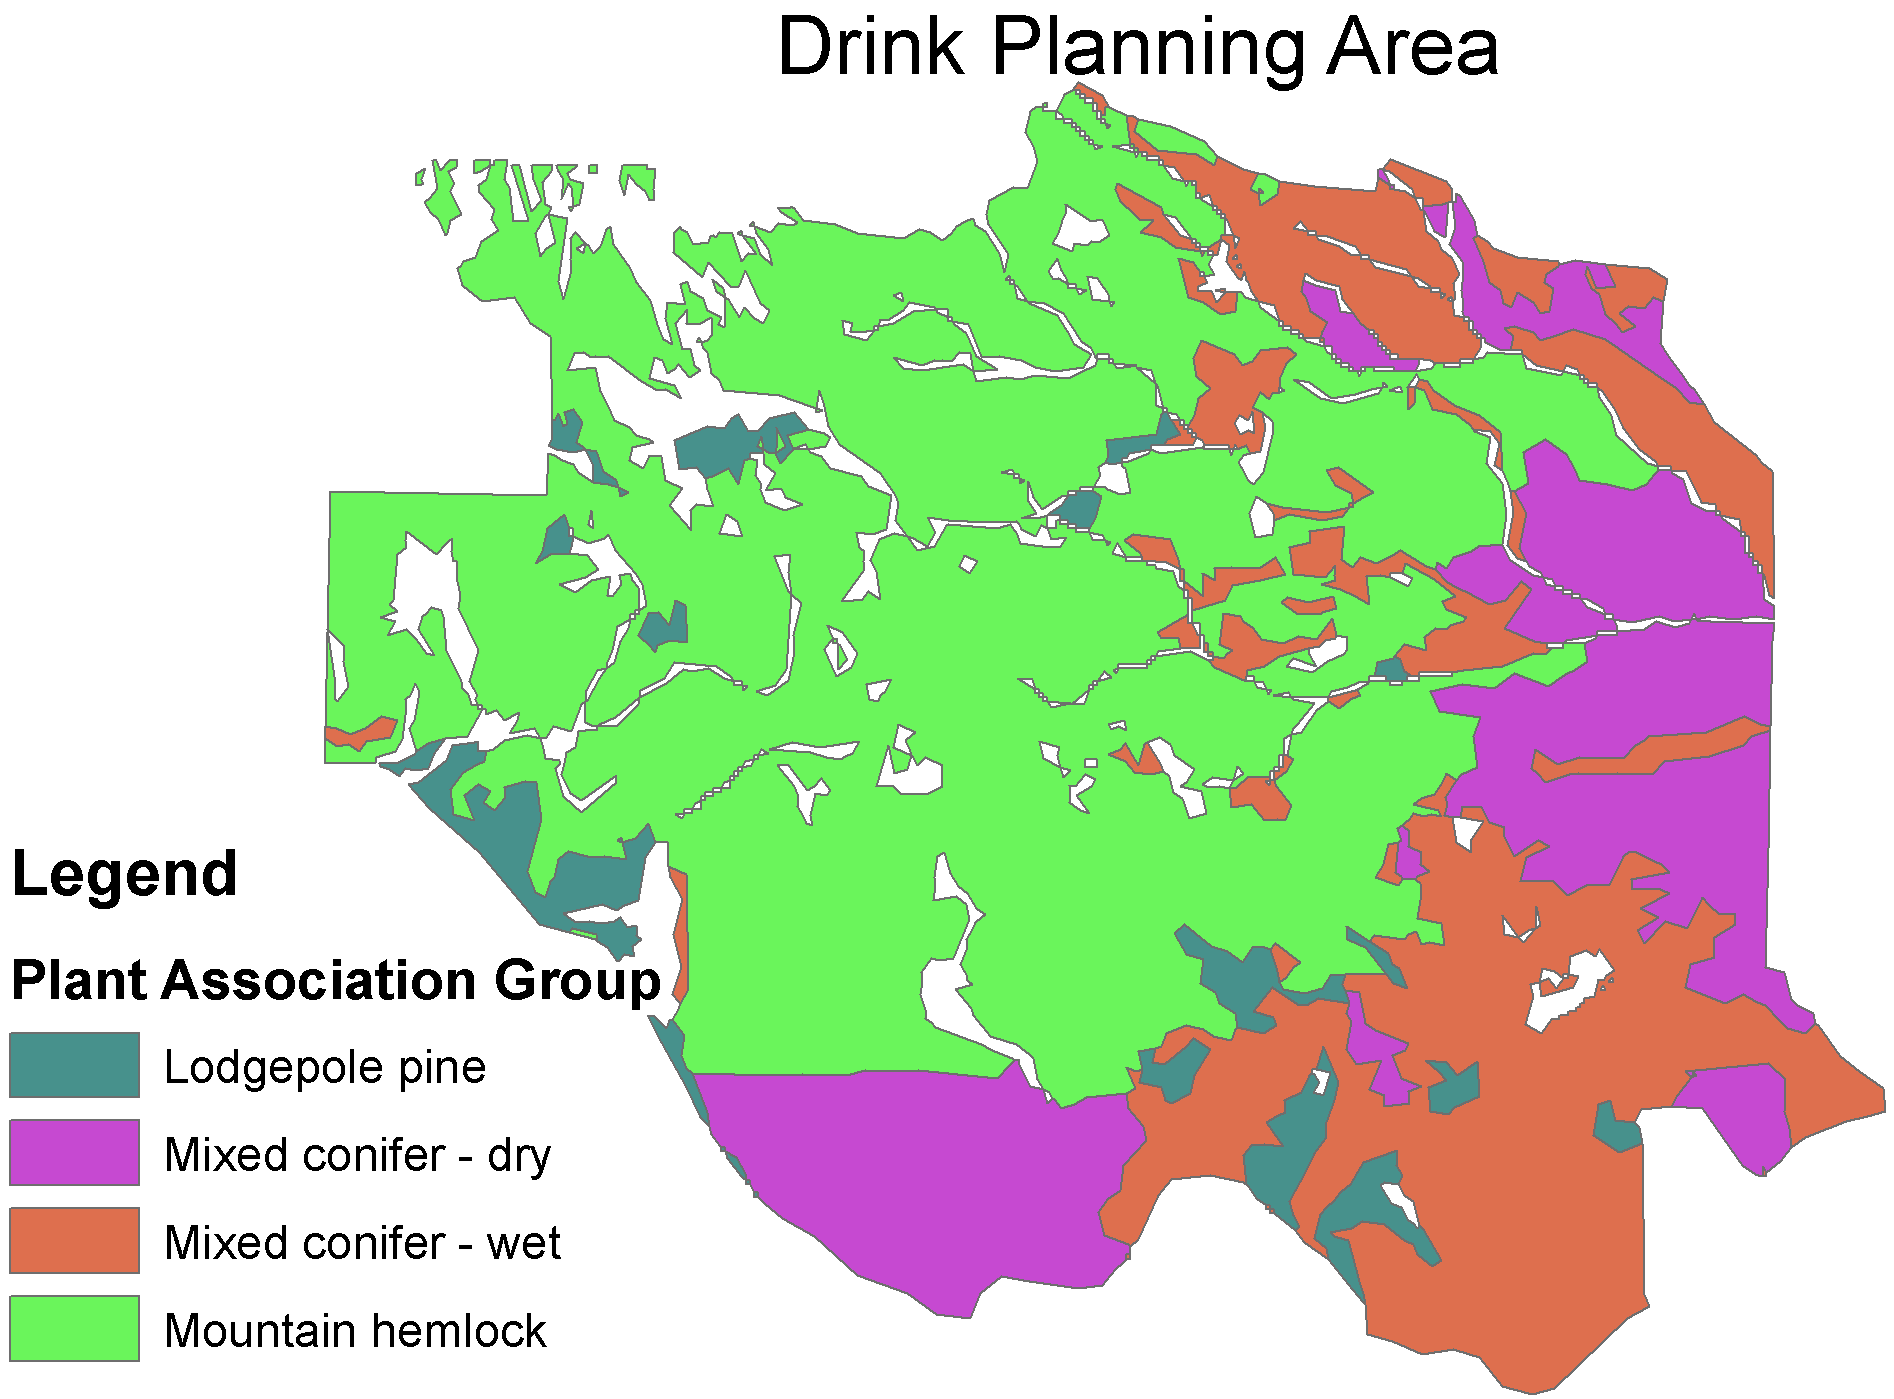
\includegraphics[width=.5\textwidth]{../images/DrinkMap_PAGs}
\caption[Plant association groups in the Drink Planning Area]{Plant association groups in the Drink Planning Area that were selected for potential treatments. Other plant association groups exist in the area but were not considered for treatment.}
\label{fig:drinkPAGs}
\end{figure}

To assess the treatments' long-term efficacy, I measured the fire hazard of the Drink at the end of an 80-year planning horizon (2015-2095). I measured the area of NSO habitat at the end of each planning period to ensure that the application of treatments did not negatively impact the habitat available for the NSO. Finally, the short-term sediment contributions from performing the treatments were measured at the time of treatment, which is assumed to be at the midpoint year in the planning period (2025 for period 1, 2045 for period 2). The planning horizon including the time of these events is shown in Figure \ref{fig:drinkPlanningHorizon}.

\begin{figure}
\centering
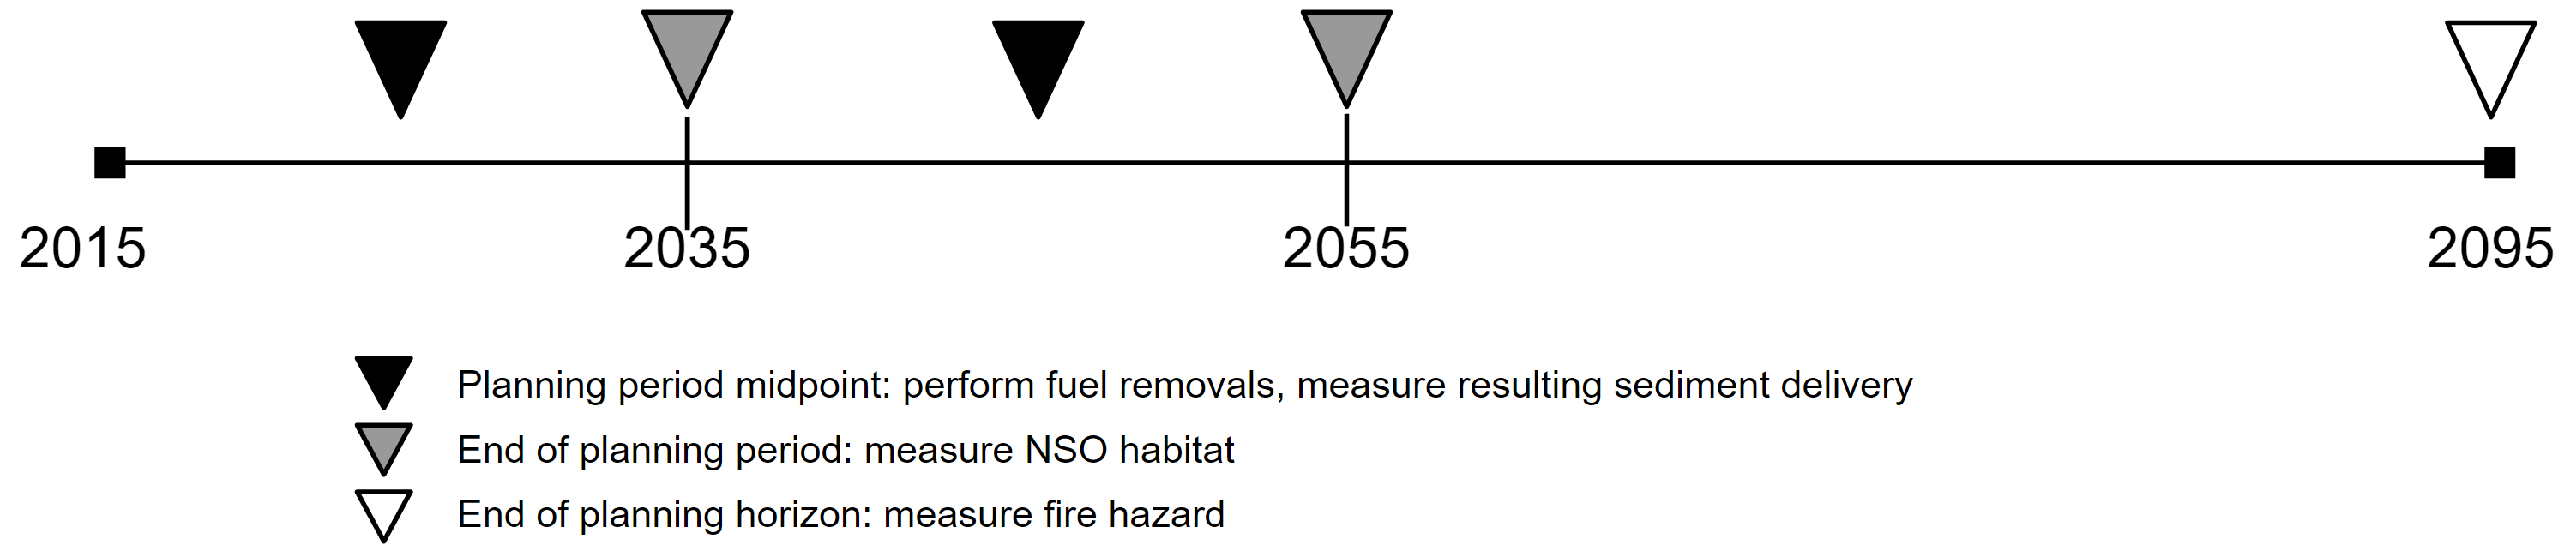
\includegraphics[width=.85\textwidth]{../images/Drink_PlanningHorizon_Sketch}
\caption[Planning horizon schematic]{The planning horizon used in the analysis spans the 80 year period from 2015 to 2095. Treatments may be performed in the first period, the second period, both, or neither. Treatments are assumed to be performed at the mid-point years of each period (black triangles). Sediment delivery is measured on treatment years. Stands' suitability for NSO habitat is measured at the end of the planning periods (gray triangles), and stands' fire hazard ratings are measured at the end of the planning horizon (white triangle).}
\label{fig:drinkPlanningHorizon}
\end{figure}

The three objectives are inherently in conflict with one another: fuel treatments drive short-term peaks in sediment delivery and potentially reduce owl habitat; minimizing short-term sediment delivery entails fewer treatments and therefore a higher fire hazard; maximizing owl habitat may require forgoing fuel treatments and again lead to higher fire hazard. In this study, I will determine how climate change impacts the tradeoffs that exist among these objectives.

\subsection{Climate Scenarios Considered}
To determine the impacts of climate change on the tradeoff structure between ecosystem services, it is first necessary to define how the impacts of climate change will be captured in the analysis. Here I use the method employed by the IPCC, namely, a scenario analysis. In a scenario analysis, multiple alternative futures are considered and no prediction is made as to which scenarios are more likely than others. There is no attempt to quantify the probability of realization of any one scenario, much like how IPCC does not attempt to quantify the probability that any particular climate model is the correct prediction of the future climate.

The alternative future climates I consider here are climate scenarios from the IPCC's Fifth Assessment \cite{ipcc2013climate}. Given the large number of potential future climates considered by the IPCC (see \cite{ipccListOfAR5Models}) combined with the computational complexity involved in the study of each one, I selected a small subset of  future climate scenarios for my analysis. I will refer to these three scenarios as ``None'', ``Ensemble RCP 4.5'', and ``Ensemble RCP 8.5''.

The first scenario, ``None'', is the assumption of no climate change. While the number of studies incorporating climate change is increasing, this is still the assumption used for many modern studies such as \cite{svetlanaDissertation2013}, from which this study is derived. Because it has served as the basis for many studies and assumes a static environment resembling today's, the ``None'' climate scenario serves as a good control against which to compare the other two climate scenarios.

As their names suggest, the second and third scenarios are ensembles. Each ensemble is comprised of 17 global circulation models (GCMs) used in the IPCC's Fifth Assessment (AR5). The selection of component GCMs in the ensembles was performed by the USFS's Climate-FVS \cite{dixon2002essential} team. The list of the 17 scenarios included in the ensemble can be found in \cite{ClimateModelsInFVSEnsemble}. Each component GCM has a corresponding climate surface which contains a vector of 35 climate parameters at over 11,000 global locations for three time periods. The climate surfaces for the ensembles were created by averaging the values of all component GCMs for each climate parameter and each time period for each location. The result is a climate surface that, while temporally sparse, is spatially robust. This configuration is appropriate for use in the Drink area given its variability in elevation and slow vegetation growth.

The two ensembles are comprised of the same 17 GCMs, but the assumed representative concentration pathways (RCP) in the component GCMs differ. The RCP indicates the additional radiative forcing (in $W/m^2$) above pre-industrial levels, with higher values of forcing indicative of more severe climate change. The GCMs in the Ensemble RCP 4.5 scenario assume 4.5 $W/m^2$ of additional radiative forcing, and the GCMs in the Ensemble RCP 8.5 scenario assume 8.5 $W/m^2$ of additional radiative forcing.

I chose these three scenarios because they represent a range of predicted climate change severity, from a $0 \degree C$ warming by the year 2100 under the ``None'' scenario to a $2.6-4.8 \degree C$ warming under RCP 8.5 \cite{ipcc2013climate}.

\subsection{Determining tradeoff relationships between ecosystem services}
\label{subsec:whyUsingMultiObjModel}
Given a selection of climate scenarios, I determined the tradeoff relationships between ecosystem services under each scenario using multi-objective mathematical optimization \cite{TothFsci2009}. This approach allocates resources so as to maximize a set of objectives subject to a set of constraints on the resource allocation. The objectives here are the ecosystem services that the USFS prioritized for the Drink area (see \S \ref{subsec:studyArea}). The optimal management of these resources will be Pareto efficient and result in optimal provision of the ecosystem services.

To allocate the resources, the multi-objective optimization model assigns values to each of a set of decision variables. Here, the decision variables are on which stands and in which period to perform silvicultural treatments. This assignment is captured by the set of decision variables $x_{i,r}$. The model assigns $x_{i,r} = 1$ if stand $i \in I = \{0,1,\ldots,302\}$ (zero-indexed numbering for the 303 management units that comprise the Drink) is to be treated according to schedule $r \in R = \{0,1,2,3\}$, where
\begin{itemize}
\item $r = 0$ is the decision not to treat the stand in either period in the planning horizon,\item $r = 1$ is the decision to treat the stand in the first period,
\item $r = 2$ is the decision to treat the stand in the second period, and
\item $r = 3$ is the decision to treat the stand in both periods.
\end{itemize}
The decision of which type of treatment to perform is not handled by the model; it is determined through the vegetation characteristics as described in \S \ref{chap:appBTreatmentSpec}.

The set of constraints on the decision variables is comprised of logical constraints, accounting constraints, and those imposed by the USFS. Logical constraints include those such as that one stand cannot be assigned to both be treated in no periods and also be treated in both periods (Equation \ref{eqn:constraintOnePrescrip}). Accounting constraints track a quantity and are often used in conjunction with other constraints (or the objective function) to bound (or optimize) that quantity. See, for example, equations \ref{eqn:constraintAreaAcctg1} and \ref{eqn:constraintAreaRestr1}. Finally, constraints imposed by the USFS include those such as labor restrictions limiting the number of hectares that may be treated in a planning period (such as Equations \ref{eqn:constraintAreaRestr1} and \ref{eqn:constraintAreaRestr2}).

I built a multi-objective model for each of the three climate scenarios. The result of each is a set of Pareto efficient solutions, each of which details a set of management actions to perform in order to attain a certain achievement in the three ecosystem services. Studying the solutions' achievements in the ecosystem services allows provides information on the tradeoff relationships between them.

\subsubsection{Acquisition and projection of data}
In order to formulate the models, I had to first acquire data. The data required included - for each climate scenario, each time period and each stand - a measure of fire hazard rating, determination of suitability for NSO habitat, and the amount of sediment deposited in the municipal watershed as a result of performing the silvicultural treatments.

For a measure for fire hazard rating, I chose the one employed by Kushch in CITESVETLANA'SMSWHENAVAILABLE. This metric suited this study, because it was developed specifically for the Drink area and was deemed appropriate by the Drink's fire specialist. This metric uses a combination of fire characteristics from Anderson's fuel models \cite{anderson1982aids} to assign a fire hazard rating: flame length, rate of spread, and total fuel load. I extended the rating system to include fuel models in this study that were not present in CITESVETLANA'SMSWHENAVAILABLE. See Table \ref{tab:firehazards}.

\begin{table}[]
\centering
\resizebox{\textwidth}{!}{%
\begin{tabular}{l|c|crrr}
\multicolumn{1}{c|}{Fuel Model} & \multicolumn{1}{c|}{\textbf{Fire Hazard}} & \multicolumn{1}{c}{Group} & \multicolumn{1}{c}{Flame length (m)} & \multicolumn{1}{c}{Rate of spread (m/hr)} & \multicolumn{1}{c}{Total fuel load (tons/ha)} \\ \hline
4*                              & \textbf{5}                                       & Shrub                     & 5.79                                 & 1508.76                                   & 32.12                                         \\
5                               & \textbf{4}                                       & Shrub                     & 1.22                                 & 362.10                                    & 8.65                                          \\
8                               & \textbf{1}                                       & Timber                    & 0.30                                 & 32.19                                     & 12.36                                         \\
9*                              & \textbf{2}                                       & Timber                    & 0.79                                 & 150.88                                    & 8.65                                          \\
10                              & \textbf{2}                                       & Timber                    & 1.46                                 & 158.92                                    & 29.65                                         \\
11*                             & \textbf{2}                                       & Logging Slash             & 1.07                                 & 120.7                                     & 28.42                                         \\
12                              & \textbf{4}                                       & Logging Slash             & 2.44                                 & 261.52                                    & 85.50                                         \\
13                              & \textbf{5}                                       & Logging Slash             & 3.20                                 & 271.58                                    & 143.57                                       
\end{tabular}%
}
\caption[Fire hazard ratings used in multi-objective model]{Fire hazard rating system used here, originally employed by CITESVETLANA'SMSWHENAVAILABLE.\\
* denotes fuel models in the extended set, not present in CITESVETLANA'SMSWHENAVAILABLE.\\
The fuel model column refers to the Anderson fuel model ratings \cite{anderson1982aids}.}
\label{tab:firehazards}
\end{table}

To determine the initial fire hazard ratings of each stand, I used the 2012 GNN structure map (\url{http://lemma.forestry.oregonstate.edu/data/structure-maps}) from Oregon State University's Landscape Ecology, Modeling, Mapping \& Analysis (LEMMA) group. The LEMMA group provides this data in a format compatible with the USFS's Forest Vegetation Simulator (FVS). I mapped the plots from the LEMMA database to the stands in the Drink area in order to produce tree and stand lists. I used these lists with FVS's database extension to import this data into FVS and then used Climate-FVS with the Fire and Fuels Extension\cite{reinhardt2003fire} (FFE) to simulate the stands' vegetation forward 80 years under each climate scenario. The output provides the fire characteristics necessary to compute the fire hazard ratings.

NSO habitat suitability was determined according to the following characteristics as specified by the USFS. Any area meeting the following would be considered ideal NSO habitat:
\begin{enumerate}
\item elevation less than 1830 m
\item the presence of trees with DBH no less than 76 cm
\item canopy closure of at least 60\%
\item greater than 200 ha in size
\end{enumerate}
I attained a digital elevation model from the US Department of Agriculture's GeoSpatial Data Gateway to compute average stand elevation and check for the first criterion. I checked the second and third criteria using the vegetation data produced by FVS. If the first three criteria are met but the area is less than 200 ha in size, it is still classified as NSO habitat but is penalized by a factor of $e = 0.5$. Since stands were generally less than 200 ha in size, the last criterion required the enumeration of all clusters of stands whose combined contiguous area exceeded 200 ha. The model checks whether all stands in such a cluster meet the first three criteria to determine whether the penalization is required.

I obtained the required data on sediment delivery using the Watershed Erosion Prediction Project (WEPP) online GIS tool \cite{frankenberger2011development}. This tool takes as input soil textures, treatment types, years of simulation, and custom climate data. I obtained soil texture data for the Drink area from the USDA's Soil Survey Geographic (SSURGO) database. Treatment types are those specified in \S \ref{chap:appBTreatmentSpec}, and the years of simulation correspond to the treatment years in the model's planning horizon.

The climate data used in the Climate-FVS and WEPP simulations was obtained through the Climate-FVS climate data server \cite{climateFVSReadyData}.

\subsubsection{The Multi-objective Optimization Model}
The first objective in the model is to minimize the cumulative fire hazard rating of the Drink area at the end of the 80-year planning horizon:
\begin{align}
Minimize \quad & F = \sum_{i\in I} \sum_{r\in R} F_{i,r} x_{i,r} \label{eqn:objFire}
\end{align}
In equation \eqref{eqn:objFire}, I sum over all stands $i \in I$ and all treatment prescriptions $r \in R$ to obtain a cumulative fire hazard metric $F$, which measures the total fire hazard rating of the Drink area at the end of the planning horizon. The coefficients $F_{i,r}$ are the area-weighted fire hazard ratings for each stand $i \in I$ at the end of the planning horizon if stand $i$ is assigned to treatment prescription $r \in R$.

The second objective is to minimize the peak short-term sediment delivery that results from performing treatments in either period one ($S_1$) or period two ($S_2$):
\begin{align}
Minimize \quad S = \max \{S_1,S_2\} \label{eqn:objSediment}
\end{align}

The last objective is to maximize the minimum area of northern spotted owl habitat at the end of each planning period, $O_1$ and $O_2$, for periods 1 and 2, respectively.
\begin{align}
Maximize \quad O = \min \{O_1,O_2\} \label{eqn:objOwl}
\end{align}

The objectives are subject to the following constraints. First, I defined the accounting variables for the area of NSO habitat available at the end of each planning period:
\begin{align}
\sum_{i\in I_{\omega,1}} \left(a_i p_{i,1} + e a_i \left( \sum_{j \in R_{i,1}} x_{i,j}-p_{i,1} \right) \right) = O_1 \label{eqn:constraintOwl1}\\
\sum_{i\in I_{\omega,2}} \left(a_i p_{i,2} + e a_i \left( \sum_{j \in R_{i,2}} x_{i,j}-p_{i,2} \right) \right) = O_2 \label{eqn:constraintOwl2}
\end{align}
The set of stands in the sum $i \in I_{\omega,t}$ are those that meet the first three criteria for NSO habitat under at least one treatment prescription $j \in R_{i,t}$, where $R_{i,t}$ is the set of treatment prescriptions for stand $i$ such that it meets the first three NSO habitat criteria at the end of planning period $t$ (where $t \in \{1,2\}$). If a stand $i$ does not meet these criteria under any treatment prescriptions (if the set $R_{i,t} = \{\emptyset\}$), then $i \notin I_{\omega,t}$. If the model assigns a stand $i \in I_{\omega,t}$ a treatment prescription $j \in R_{i,t}$, then stand $i$ meets the first three NSO habitat criteria at the end of planning period $t$, and the variable $x_{i,j}=1$. If, in addition, the stand $i$ is part of a cluster of stands all meeting the first three NSO habitat criteria at the end of period $t$ and whose combined contiguous area is greater than 200 ha, then the variable $p_{i,t} = 1$. Notice that when $p_{i,t} = 0$, the stand's contribution is discounted by $e = 0.5$, and when $p_{i,t} = 1$ it is not.

Next, I defined the accounting variables for the sediment delivery that results from the performance of the prescribed management actions in each planning period.
\begin{align}
\sum_{i\in I} \sum_{r\in 1,3} s_{i,1} x_{i,r} = S_1 \label{eqn:constraintSediment1}\\
\sum_{i\in I} \sum_{r\in 2,3} s_{i,2} x_{i,r} = S_2 \label{eqn:constraintSediment2}
\end{align}
The coefficients $s_{i,t}$ are the amount of sediment (in tonnes) that would result from treating stand $i$ in time period $t$.

In order to control the trigger variables $p_{i,t}$ indicating a stand's inclusion in a 200 ha cluster of NSO habitat at the end of period $t$, I used the following two constraints:
\begin{align}
\sum_{i \in D_c} \sum_{j \in R_{i,t}} x_{i,j} - |c| q_{c,t} &\ge 0 \qquad \forall t \in \{1,2\}, c \in C \label{eqn:constraintClusterTriggers}\\
\sum_{c \in C_i} q_{c,t} - p_{i,t} &\ge 0 \qquad \forall t \in \{1,2\}, i \in I_{\omega,t} \label{eqn:constraintPVarTriggers}
\end{align}
$c \in C$ are the clusters of stands whose combined area is greater than 200 ha. A cluster $c$ contains the set of stands $i \in D_c$. Equation \eqref{eqn:constraintClusterTriggers} specifies that all stands $i \in D_c$ within a cluster $c \in C$ must be assigned a management prescription such that they meet all NSO habitat criteria at the end of planning period $t$ in order for the cluster trigger variable $q_{c,t}$ to take value 1.

Equation \eqref{eqn:constraintPVarTriggers} specifies that if no cluster $c \in C_i$ - the set of clusters that contain site $i$ - meets NSO qualifications at the end of period $t$, then the trigger variable $p_{i,t}$ must take value 0. If a cluster $c \in C_i$ does meet NSO qualifications at the end of planning period $t$, then the sense of the NSO objective function \eqref{eqn:objOwl} will draw up the value of the variable $p_{i,t}$ to 1.

I also imposed the logical restriction that each stand may be assigned to at most one treatment prescription.
\begin{align}
\sum_{r \in R} x_{i,r} = 1  \qquad \forall i \in I \label{eqn:constraintOnePrescrip}
\end{align}

Next, I ensured that the area treated in each time period is less than a pre-specified maximum area $A$. Here I used a value of $A = 6000$ acres, or 2428 ha:
\begin{align}
\sum_{i \in I} \sum_{r \in 1,3} a_i x_{i,r} &= H_1 \label{eqn:constraintAreaAcctg1}\\
\sum_{i \in I} \sum_{r \in 2,3} a_i x_{i,r} &= H_2 \label{eqn:constraintAreaAcctg2}\\
H_1 &\le A \label{eqn:constraintAreaRestr1}\\
H_2 &\le A \label{eqn:constraintAreaRestr2}
\end{align}
Equations \ref{eqn:constraintAreaAcctg1} and \ref{eqn:constraintAreaAcctg2} define the accounting variables for the areas treated in time periods 1 and 2, $H_1$ and $H_2$, and equations \ref{eqn:constraintAreaRestr1} and \ref{eqn:constraintAreaRestr2} impose the upper bound.

Finally, I specified fluctuation constraints to bound the difference in the area treated in each time period:
\begin{align}
\ell H_1 - H_2 &\le 0 \label{eqn:constraintAreaFlucL}\\
-u H_1 + H_2 &\le 0 \label{eqn:constraintAreaFlucU}
\end{align}
I defined a maximum of 20\% areal fluctuation between the time periods. That is, $\ell = 0.8$ and $u = 1.2$.

Together with the binary specifications on the variables (equation \eqref{eqn:constraintNonNeg}), the complete model is
\begin{align*}
Minimize \quad & \\
F=&\sum_{i\in I}\sum_{r\in R} F_{i,r} x_{i,r}\\
S=&\max \{S_1,S_2\}\\
Maximize \quad & \\
O =&\min \{O_1,O_2\}
\end{align*}

Subject to:
\begin{align}
\sum_{i\in I_{\omega,t}} \left(a_i p_{i,t} + e a_i \left( \sum_{j \in R_{i,t}} x_{i,j}-p_{i,t} \right) \right) &= O_t \qquad \forall t \in \{1,2\} \notag\\
\sum_{i\in I} \sum_{r\in 1,3} s_{i,r} x_{i,r} &= S_1 \notag\\
\sum_{i\in I} \sum_{r\in 2,3} s_{i,r} x_{i,r} &= S_2 \notag\\
\sum_{i \in D_c} \sum_{j \in R_{i,t}} x_{i,j} - |c| q_{c,t} &\ge 0 \qquad \forall t \in \{1,2\}, c \in C \notag\\
\sum_{c \in C_i} q_{c,t} - p_{i,t} &\ge 0 \qquad \forall t \in \{1,2\}, i \in I_{\omega,t} \notag\\
\sum_{r \in R} x_{i,r} &= 1  \qquad \forall i \in I \notag\\
\sum_{i \in I} \sum_{r \in 1,3} a_i x_{i,r} &= H_1 \notag\\
\sum_{i \in I} \sum_{r \in 2,3} a_i x_{i,r} &= H_2 \notag\\
H_t &\le A \qquad \forall t \in \{1,2\} \notag\\
\ell H_1 - H_2 &\le 0 \notag\\
-u H_1 + H_2 &\le 0 \notag\\
x_{i,r}, p_i, q_c \in \{0,1\} \quad &\forall i \in I, r \in R, c \in C \label{eqn:constraintNonNeg}
\end{align}

\subsection{Model solution}
In general, solving a bounded and non-degenerate multi-objective optimization problem with $N$ objectives produces a set of objective vectors (also called ``solutions'') $\mathbf{z} \in Z$ where $\mathbf{z}=\braket{z^1,\ldots,z^N}$. The set of solutions $Z$ is referred to as the Pareto-optimal frontier or efficient frontier or, simply, frontier. The solutions comprising an efficient frontier have the special relationship such that no component of a solution $\mathbf{z}^i$ can be improved upon without one of the other components $\mathbf{z}^j$ ($j \neq i$) degrading. This quality is known as Pareto efficiency. For example, this relationship in the current problem means that further reducing the value of fire hazard in a solution would result in either additional sediment deposits, a reduction of NSO habitat, or both.

Thus the efficient frontier provides information on the tradeoff structure that exists between ecosystem services. Parameterizing and solving the above model for each of the climate scenarios generates three frontiers: $Z_{\text{None}}$, $Z_{4.5}$, and $Z_{8.5}$ for the None, Ensemble RCP 4.5, and Ensemble RCP 8.5 scenarios, respectively. Since climate is the only thing that differs between the models and their resulting frontiers, comparing the frontiers provides insight into how climate impacts the tradeoff structures between the ecosystem services.

To solve the models, I wrote my own implementation of T\'{o}th's Alpha-Delta algorithm \cite{TothThesis} utilizing the IBM ILOG CPLEX optimization engine. The Alpha-Delta algorithm finds the optimal set $Z$ by iteratively slicing the $N$-dimensional objective space with a tilted $N-1$ dimensional plane. To derive the frontiers, I used an alpha parameter of $\alpha = .01$ and delta parameters of $\delta_{Hab} = 1$ ha and $\delta_{Sed} = 2$ tonnes for the NSO habitat and sediment delivery objectives, respectively.

\subsection{Comparing Tradeoffs under each Climate Change Scenario}
By parameterizing and solving the multi-objective model once for each climate scenario, I generated three efficient frontiers. To determine the impact of climate on tradeoffs in ecosystem services, I compared these frontiers and the level of conflict between the objectives within each of them. However, no standardized procedure exists for this task. In order to make comparisons at the frontier (climate scenario) level, I drew on methods used in the field of evolutionary multi-objective optimization (EMO). To address conflict between objectives within a frontier, I applied a method used for objective pruning in many-objective optimization and a variant of a method used in EMO.

\subsubsection{Comparing frontiers}
Researchers in the field of EMO develop algorithms to generate a set of non-dominated solutions that best represents the true Pareto-optimal frontier \cite{deb2001multi}. To test their algorithms, they solve a benchmark multi-objective optimization problem and compare their resulting frontiers to the known Pareto front for that problem \cite{knowles2002metrics}. There is no assurance of optimality of the solutions derived using these algorithms, so they require a means of comparing the resulting frontiers to determine if one algorithm produces a ``better'' non-dominated frontier than another. Zitzler et al. provide a review of comparison methods in \cite{zitzler2003performance}. These methods aim to quantify certain traits about a frontier that can be used to measure their success in approximation of the true frontier.

My motivation in comparing frontiers is different from EMO in that, rather than comparing frontiers that result from solving identical models with varying methods, I compared frontiers that result from solving varying models (albeit with the same structure) with identical methods. The primary difference in the output of my approach compared to EMO is the assured optimality of the solutions in my frontiers. Because of this difference, not all comparison methods are applicable. For instance, the indicator for the number of Pareto points contained in the frontier does not make sense in my case, since all points on my frontiers are Pareto-optimal. Despite the difference, however, other comparison methods still have value. I chose a subset of these methods to compare my frontiers: the additive binary epsilon and binary hypervolume indicators, and the unary distance, additive unary epsilon, unary hypervolume, and unary spacing indicators.

Some methods for comparing frontiers require the normalization of the objective space. This is because the climate scenarios alter the bounds on the achievable values of the ecosystem services, resulting in frontiers whose objective spaces do not overlap.

In my analysis and in the definitions that follow, I chose the normalization such that all objectives are maximized, and each frontier is contained within the unit hypercube. That is, each objective is bounded between 0 and 1, yielding a frontier bounded by $[0,1]^N$. Defining the nadir solution $\mathbf{z}_{\text{nad}}$ of a frontier of points $z \in Z$ as the objective vector with components
\begin{align}
\mathbf{z}_{\text{nad}}^i = \inf_{z} \{ z^i \} \quad \forall 1 \le i \le N
\end{align}
and the ideal solution as the objective vector with components
\begin{align}
\mathbf{z}_{\text{ideal}}^i = \sup_{z} \{ z^i \} \quad \forall 1 \le i \le N
\end{align}
then under my normalization, the nadir solution is the origin and the ideal solution is the $N$-dimensional vector of ones $\mathbf{1}_N$.

The definitions of dominance terms used here are in Table \ref{tab:dominanceRelations}.

\begin{table}[ht]
\centering
\resizebox{\textwidth}{!}{%
\begin{tabular}{|p{.2\linewidth}|p{.1\linewidth}|p{.3\linewidth}|p{.1\linewidth}|p{.3\linewidth}|}
\hline
\textbf{Relation}           & \multicolumn{2}{c|}{\textbf{Solutions}}                                                                                                                                                                          & \multicolumn{2}{c|}{\textbf{Frontiers}}                                                                                                     \\ \hline
Strictly dominates & $\mathbf{z}_1 \succ \succ \mathbf{z}_2$ & $\mathbf{z}_1$ is better than $\mathbf{z}_2$ in all objectives                                                                                  & $Z_1 \succ \succ Z_2$ & Every solution in $Z_2$ is strictly dominated by at least one solution in $Z_1$                  \\ \hline
Dominates          & $\mathbf{z}_1 \succ \mathbf{z}_2$       & $\mathbf{z}_1$ is better than $\mathbf{z}_2$ in at least one objective and is not worse in any objective & $Z_1 \succ Z_2$       & Every solution in $Z_2$ is dominated by at least one solution in $Z_1$                           \\ \hline
Better             &                                         &                                                                                                                                                               & $Z_1 \rhd Z_2$        & Every solution in $Z_2$ is weakly dominated by at least one solution in $Z_1$ and $Z_1 \neq Z_2$ \\ \hline
Weakly dominates   & $\mathbf{z}_1 \succeq \mathbf{z}_2$     & $\mathbf{z}_1$ is at least as good as $\mathbf{z}_2$ in all objectives                                                                                        & $Z_1 \succeq Z_2$     & Every solution in $Z_2$ is weakly dominated by at least one solution in $Z_1$          \\ \hline
Incomparable       & $\mathbf{z}_1 || \mathbf{z}_2$          & Neither $\mathbf{z}_1$ nor $\mathbf{z}_2$ weakly dominates the other                                                                                          & $Z_1 || Z_2$          & Neither $Z_1$ nor $Z_2$ weakly dominates the other                                                         \\ \hline
\end{tabular}%
}
\caption[Dominance relationships for frontiers and solutions]{Definitions of dominance relationships between solutions and between frontiers, reproduced from \cite{zitzler2003performance}.}
\label{tab:dominanceRelations}
\end{table}

\paragraph{Additive binary epsilon indicator $I_{\epsilon_+2}$} Given two frontiers, $Z_1$ and $Z_2$, the additive binary epsilon indicator is defined as \cite{zitzler2003performance}
\begin{align}
I_{\epsilon_+2} (Z_1,Z_2) = \inf_{\epsilon \in \mathbb{R}} \set{\forall \mathbf{z}_2 \in Z_2 \; \exists \mathbf{z}_1 \in Z_1 : \mathbf{z}_1 \succeq_{\epsilon_+} \mathbf{z}_2}
\end{align}
where $\succeq_{\epsilon_+}$ is the additive $\epsilon$-dominance relationship:
\begin{align}
\mathbf{z}_1 \succeq_{\epsilon_+} \mathbf{z}_2 \iff \epsilon + \mathbf{z}_1^i \ge \mathbf{z}_2^i \quad \forall 1 \le i \le N
\end{align}
Intuitively, $\epsilon$ is the minimum amount by which a frontier $Z_1$ must be translated such that every solution $\mathbf{z}_2 \in Z_2$ is ``covered''. See Figure \ref{fig:binaryEpsilon}. Positive values of $I_{\epsilon_+2} (Z_1,Z_2)$ indicate the presence of points $\mathbf{z}_2 \in Z_2$ that are not dominated by $Z_1$. Negative values of $I_{\epsilon_+2} (Z_1,Z_2)$ indicate that $Z_1$ strictly dominates $Z_2$ ($Z_1 \succ \succ Z_2$).

\begin{figure}[ht]
\centering
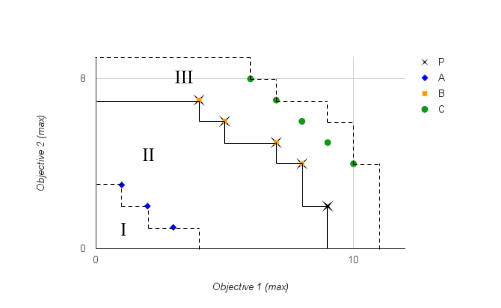
\includegraphics[width=.7\textwidth]{../images/BinaryEpsilonIndicator}
\caption[The additive binary epsilon indicator $I_{\epsilon_+2}$]{Depiction of the additive binary epsilon indicator $I_{\epsilon_+2}$ and the additive epsilon dominance relationship $\succeq_{\epsilon_+}$. In the figure,

\begin{minipage}{\linewidth}
  \begin{align*}
    I_{\epsilon_+2} (P,A) = -4 < 0 \qquad I_{\epsilon_+2} (P,B) = 0 \qquad I_{\epsilon_+2} (P,C) = 2 > 0
  \end{align*}
\end{minipage}

Region III is $\epsilon_+$-dominated for $\epsilon = 2$; region II is $\epsilon_+$-dominated for $\epsilon = 0$; region I is $\epsilon_+$-dominated for $\epsilon = -4$. Note that region II also encompasses region I, and region III encompasses region II.}
\label{fig:binaryEpsilon}
\end{figure}

\paragraph{Additive unary epsilon indicator $I_{\epsilon_+}$} I define the unary epsilon indicator as
\begin{align}
I_{\epsilon_+} (Z) = I_{\epsilon_+2} (Z,\mathbf{z}_{\text{ideal}})
\end{align}
That is, the additive unary epsilon indicator is identical to the additive binary epsilon indicator where the second frontier consists of a single point: the ideal solution for the first frontier.

This differs from the unary epsilon indicator traditionally used in EMO \cite{zitzler2003performance}. In EMO, the frontier is compared against a reference nondominated set. However, because my frontiers are optimal, there is no reference set against which to compare them.

\paragraph{Unary hypervolume indicator $I_{H1}$ and binary hypervolume indicator $I_{H2}$}
For every solution $\mathbf{z}_i$ in a frontier $Z$ define the hyperrectangle $r_i$ whose diagonal corners are the origin and the objective vector $\mathbf{z}_i = \braket{z^1,\ldots,z^N}$ (see Figure \ref{fig:frontierVolumes}). Then the unary hypervolume indicator of the frontier $Z$ is the $N$-dimensional volume of the union of all of the hyperrectangles corresponding to the solutions in $Z$:
\begin{align}
I_{H1} (Z) = \text{vol} \left( \bigcup_{i = 1}^{|Z|} r_i \right)
\end{align}
Then define the binary hypervolume indicator of two frontiers $Z_1$ and $Z_2$ as \cite{zitzler1999evolutionary}
\begin{align}
I_{H2} (Z_1,Z_2) = I_{H1} (Z_1 + Z_2) - I_{H1} (Z_2)
\end{align}
where $I_{H1} (Z_1 + Z_2)$ is the unary hypervolume indicator of the frontier consisting of the nondominated points in $Z = \{z \in Z_1 \cup Z_2\}$ . See Figure \ref{fig:binaryHypervolume}. The binary hypervolume indicator provides the volume of frontier $Z_1$ that is not contained within frontier $Z_2$. Larger values of $I_{H1}$ correspond to frontiers occupying larger amounts of the objective space. In a normalized objective space, $I_{H2}(Z_1, Z_2) > I_{H2}(Z_2, Z_1)$ indicates areas of less conflict between objectives in $Z_1$ than in $Z_2$.

\begin{figure}[ht]
\centering
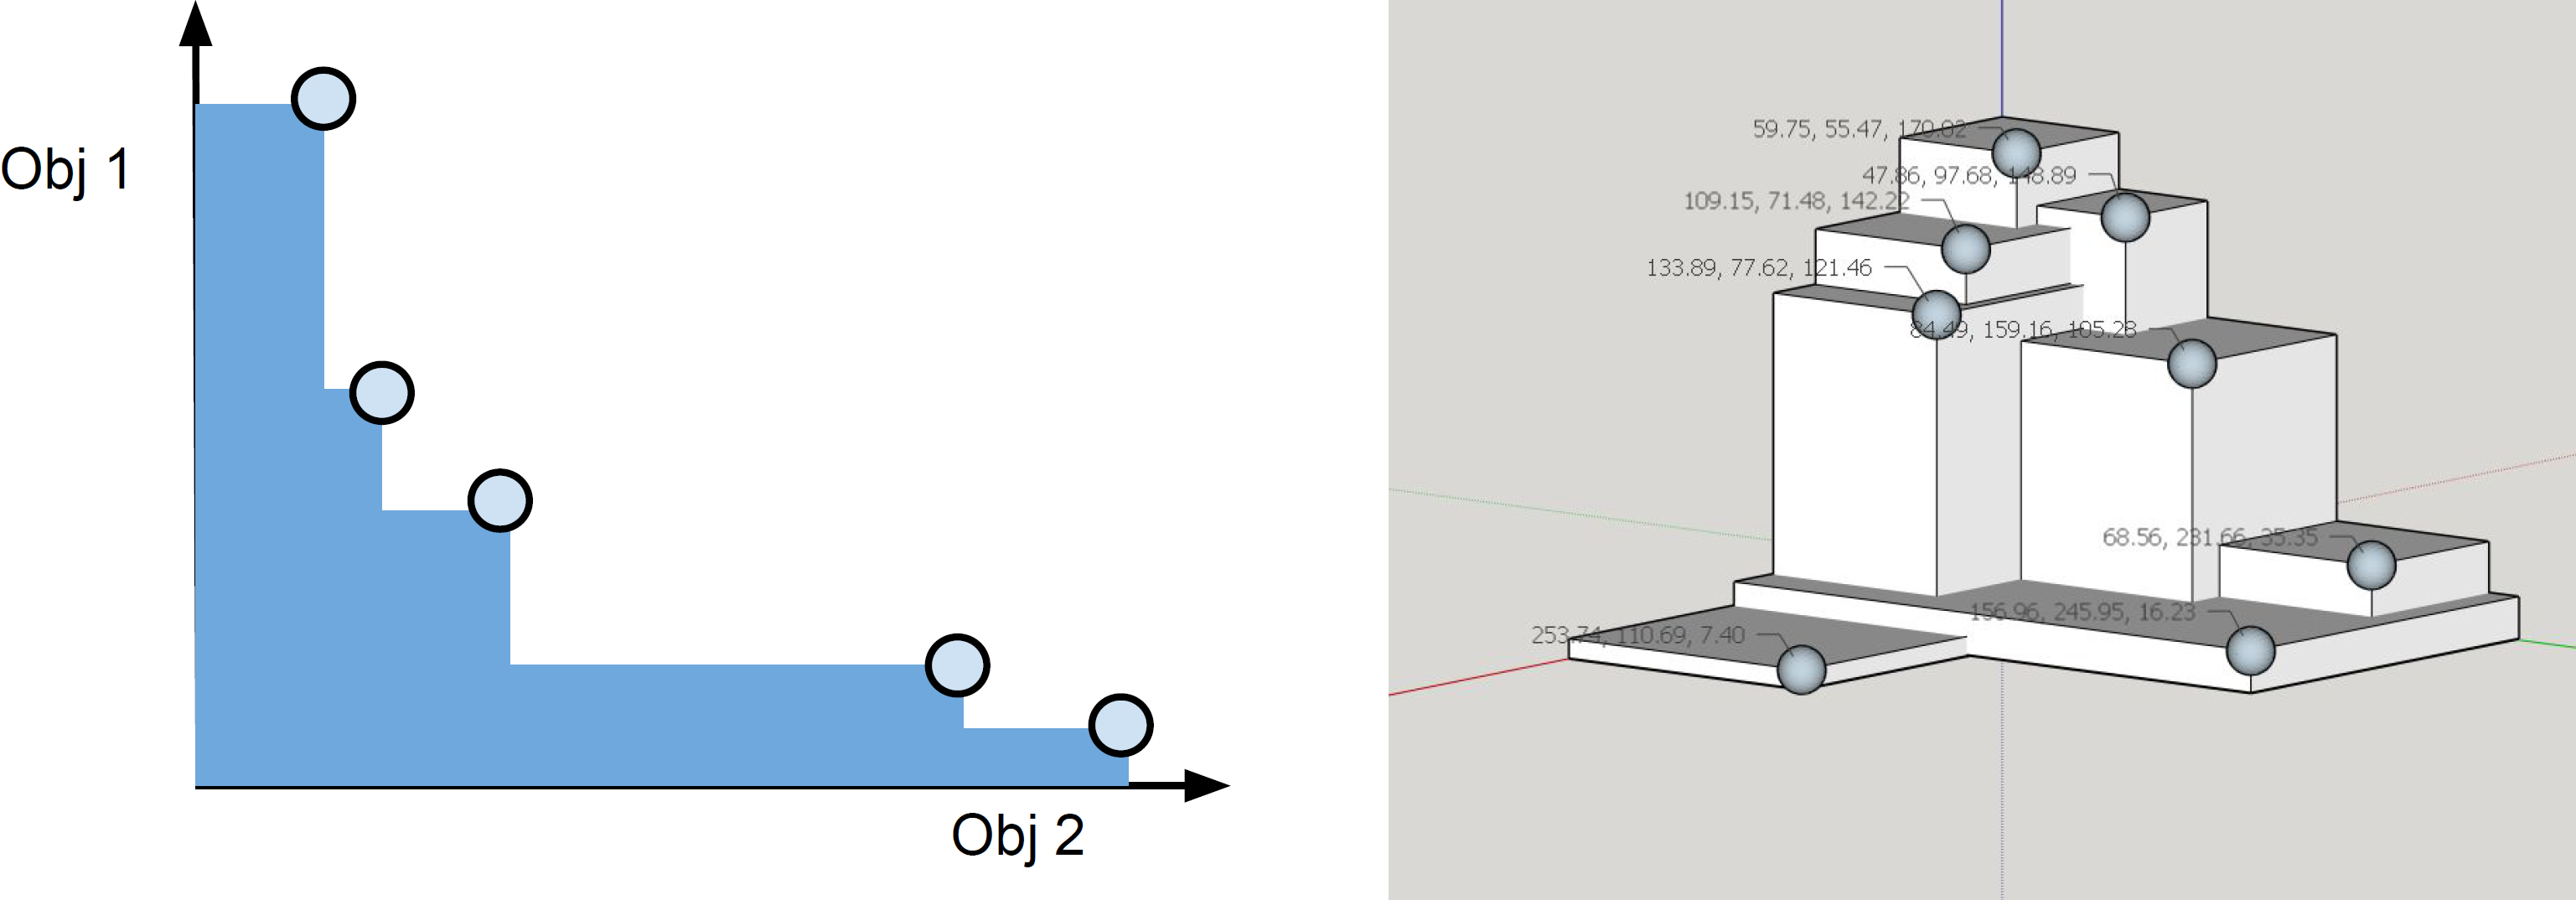
\includegraphics[width=.85\textwidth]{../images/FrontierVolumesNo2DOutlines}
\caption[Hypervolume of Pareto frontiers]{Depiction of the hypervolumes of frontiers with two objectives (left) and three objectives (right).}
\label{fig:frontierVolumes}
\end{figure}

\begin{figure}[ht!]
\centering
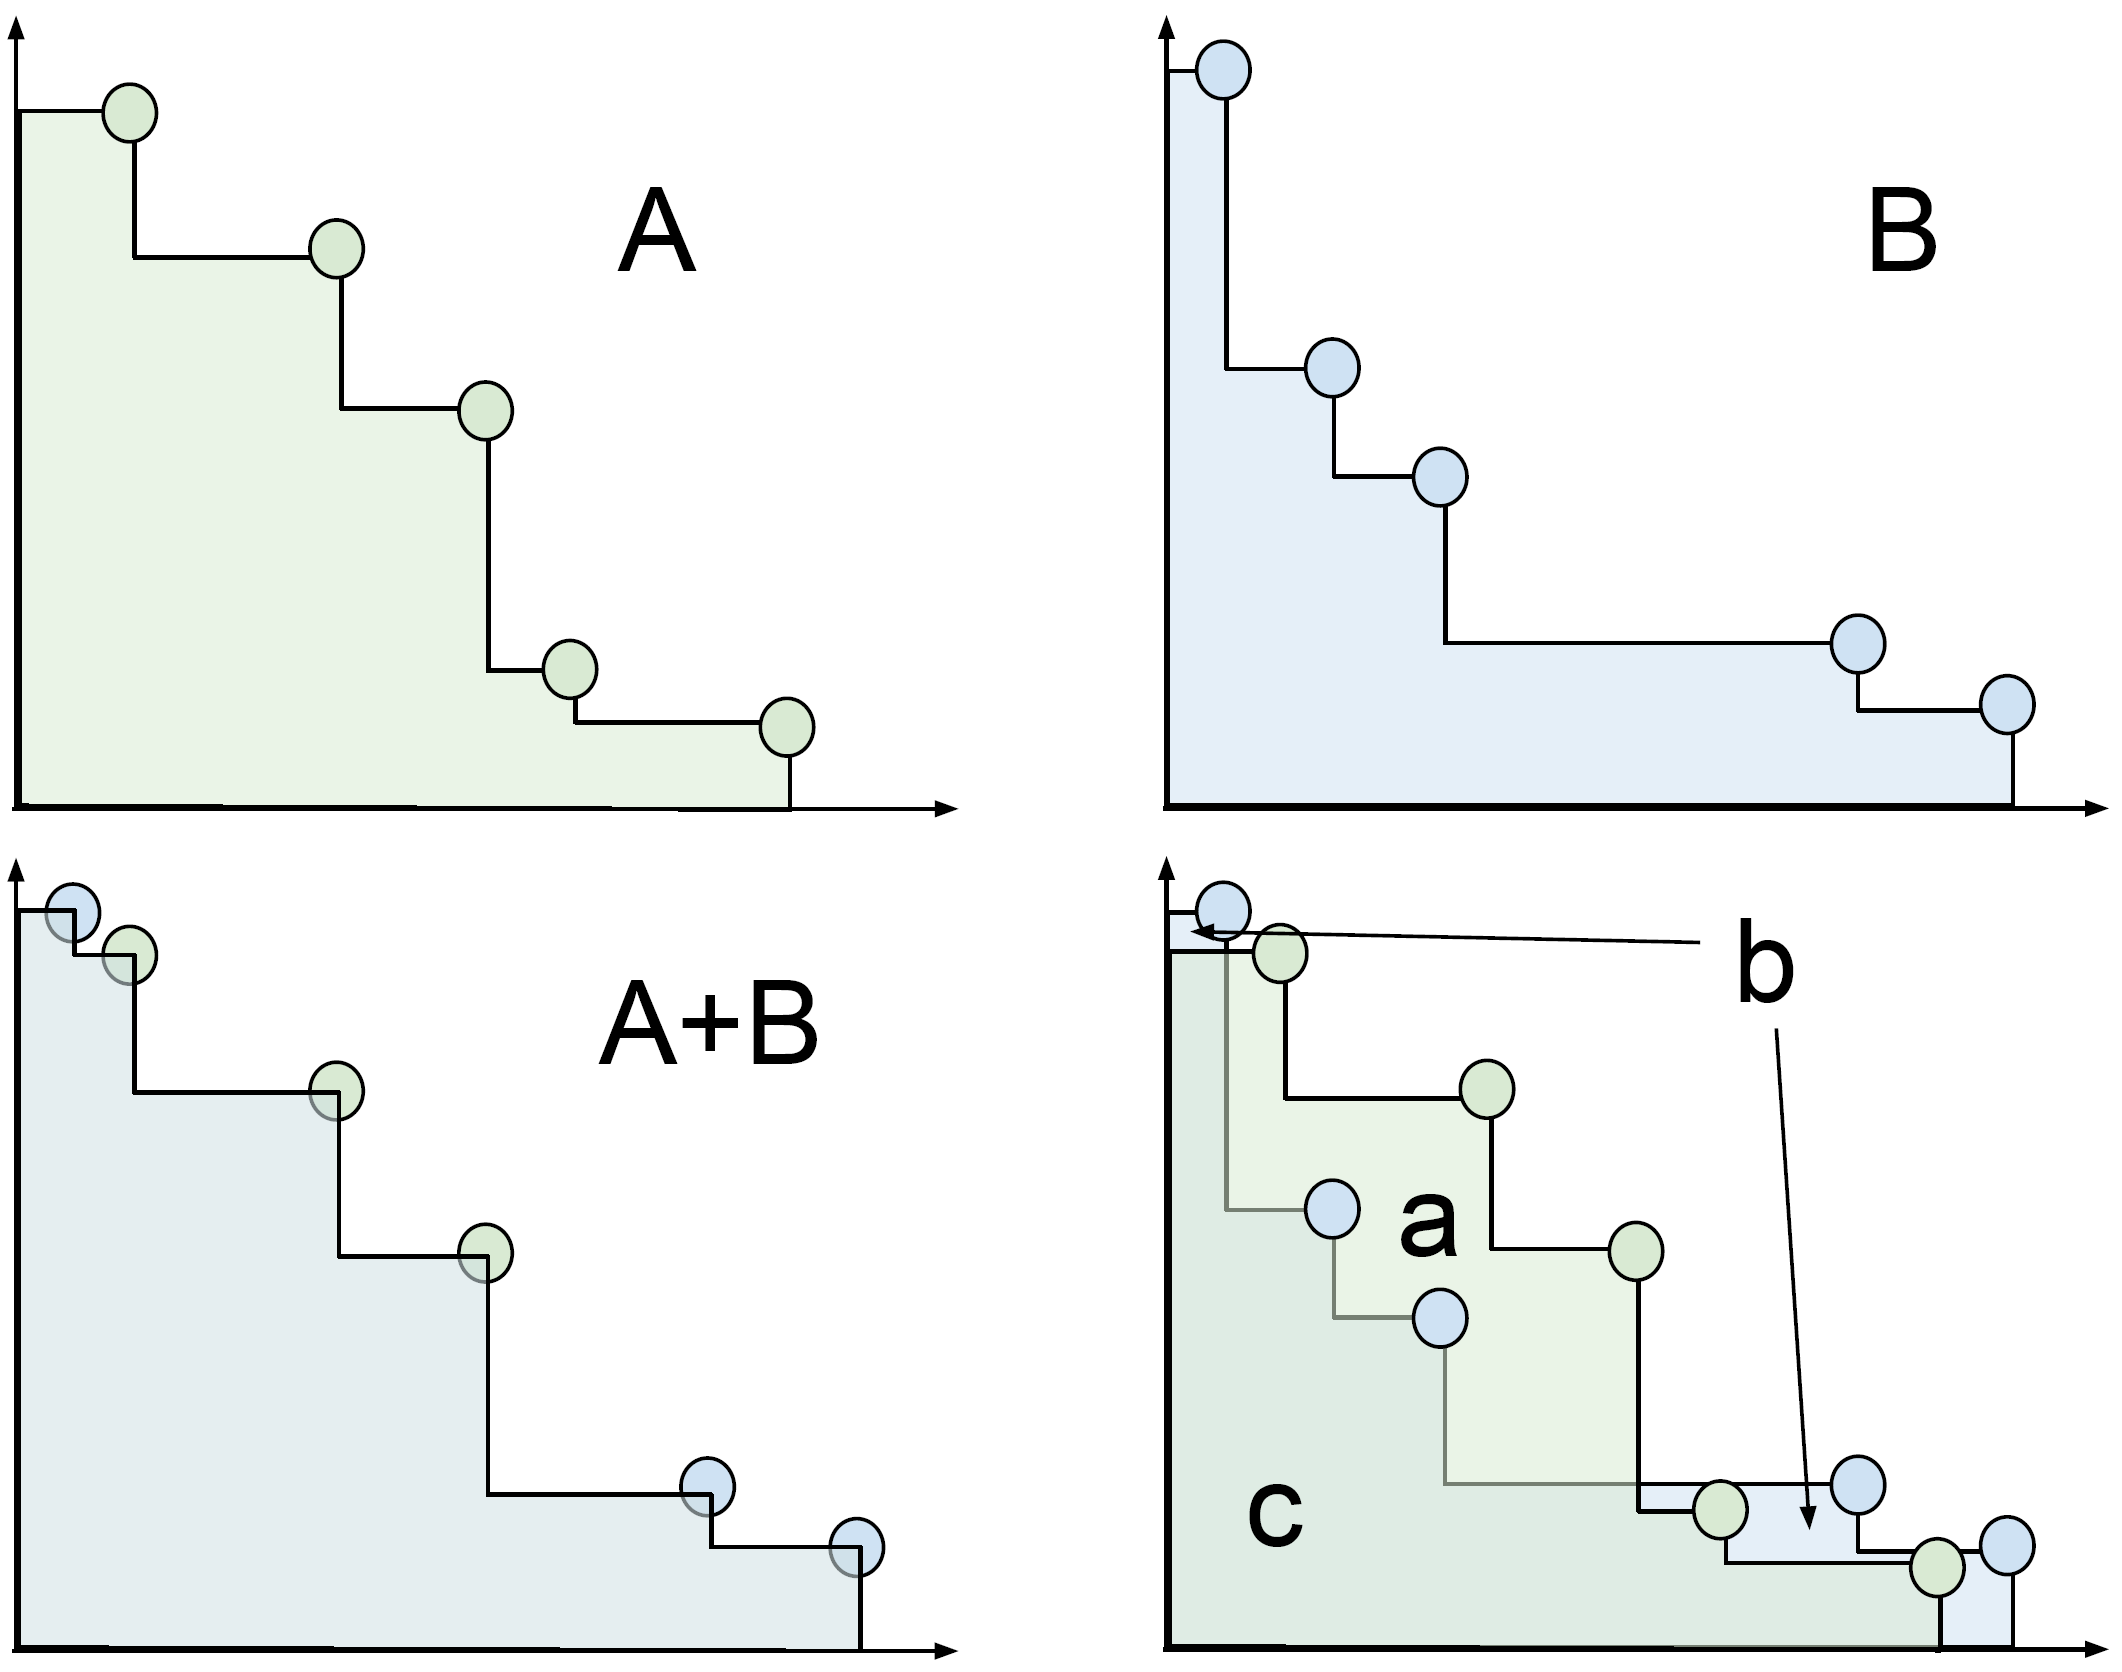
\includegraphics[width=.7\textwidth]{../images/BinaryHypervolume}
\caption[Binary hypervolume indicator]{Depiction of the binary hypervolume indicator. The individual frontiers are shown in the top row: frontier $A$ (left) and frontier $B$ (right). The merged frontier $A+B$ is shown in bottom left - note the absence of points that were dominated when combined. Following the naming of regions as shown in the bottom right figure, the binary hypervolume indicator is equal to
\begin{minipage}{\linewidth}
  \begin{align*}
    I_{H2} (A,B) = \left(\text{area}_a + \text{area}_b + \text{area}_c \right) - \left( \text{area}_b + \text{area}_c \right) = \text{area}_a
  \end{align*}
\end{minipage}%
}
\label{fig:binaryHypervolume}
\end{figure}

I developed a custom algorithm to solve for the hypervolume idicators. The details of the algorithm may be found in \S \ref{chap:appAHypervolumeAlgo}.

\paragraph{Unary distance indicator $I_d$} The unary distance indicator measures the average distance from the frontier to the ideal solution:
\begin{align}
I_d = \frac{\sum_{\mathbf{z} \in Z} ||\mathbf{z}_{\text{ideal}} - \mathbf{z} ||}{N}
\end{align}
Smaller values of $I_d$ correspond to frontiers that are closer to the ideal solution, which may imply less conflict between objectives. This metric is analogous to the unary distance indicator described in \cite{czyzzak1998pareto} and is more commonly used in EMO. Where the metric used here measures the distance to the ideal solution, the metric in \cite{czyzzak1998pareto} measures the distance to a reference Pareto frontier.

\paragraph{Unary Spacing Indicator $I_s$} The unary spacing indicator, or Schott's spacing metric\cite{schott1995fault}, computes the standard deviation of the distance between points in the frontier:
\begin{align}
I_s = \sqrt{\frac{1}{N-1} \sum_{\mathbf{z} \in Z} (d_z - \overbar{d})^2}
\end{align}
where
\begin{align}
d_z = \min_{\mathbf{y} \in Z, \mathbf{y} \neq \mathbf{z}} ||\mathbf{z} - \mathbf{y}||
\end{align}
and $\overbar{d}$ is the average over all $d_z$. In EMO, the spacing indicator provides a measure of an algorithm's ability to search the frontier space uniformly. Here, the spacing metric provides a measure of the flexibility afforded to the decision maker under each climate scenario, since smaller values of $I_s$ imply a higher density of solutions and greater flexibility.

\subsubsection{Quantifying conflict between objectives within a frontier}

The above methods provide frontier-level metrics of conflict and tradeoffs. To determine the degree of conflict between two objectives within a single frontier, we employ two techniques. The first is an approach used in many-objective optimization, and the second is a variant of the unary hypervolume indicator.

\paragraph{Pearson correlation coefficients} Given the increased difficulty in solving many-objective optimization problems \cite{khare2003performance}, researchers in this field seek to reduce the number of objectives considered in the model. To determine which objectives most strongly influence the shape of the frontier, they compute the correlation between each pair of objectives \cite{deb2005finding}. Objective pairs with strong negative correlation conflict with one another. To rank the relative conflict between objectives in each climate scenario, I compute their Pearson correlation coefficients:
\begin{align}
\rho_{X,Y} = \frac{\text{cov}(X,Y)}{\sigma(X)\sigma(Y)}
\end{align}
where, for objectives $x$ and $y$, $X$ and $Y$ are
\begin{align}
X = \{ \mathbf{z}^x_1, \mathbf{z}^x_2, \ldots, \mathbf{z}^x_{|Z|} \} \\
Y = \{ \mathbf{z}^y_1, \mathbf{z}^y_2, \ldots, \mathbf{z}^y_{|Z|} \}
\end{align}

\paragraph{Area of 2D frontier projection $A_{xy}$}
The second technique to measure the conflict between objectives within a frontier uses the unary hypervolume indicator. Given a frontier with objective vectors in $N$ dimensions, take two objectives $x$ and $y$, and project the $N$-dimensional frontier to the two-dimensional $xy$-plane. Remove solutions dominated in this projection, and compute the hypervolume indicator (which, in two-dimensions, is simply the area). See Figure \ref{fig:frontierCrossSection}. Larger values of $A_{xy}$ imply less conflict between objectives $x$ and $y$.

\begin{figure}[ht]
\centering
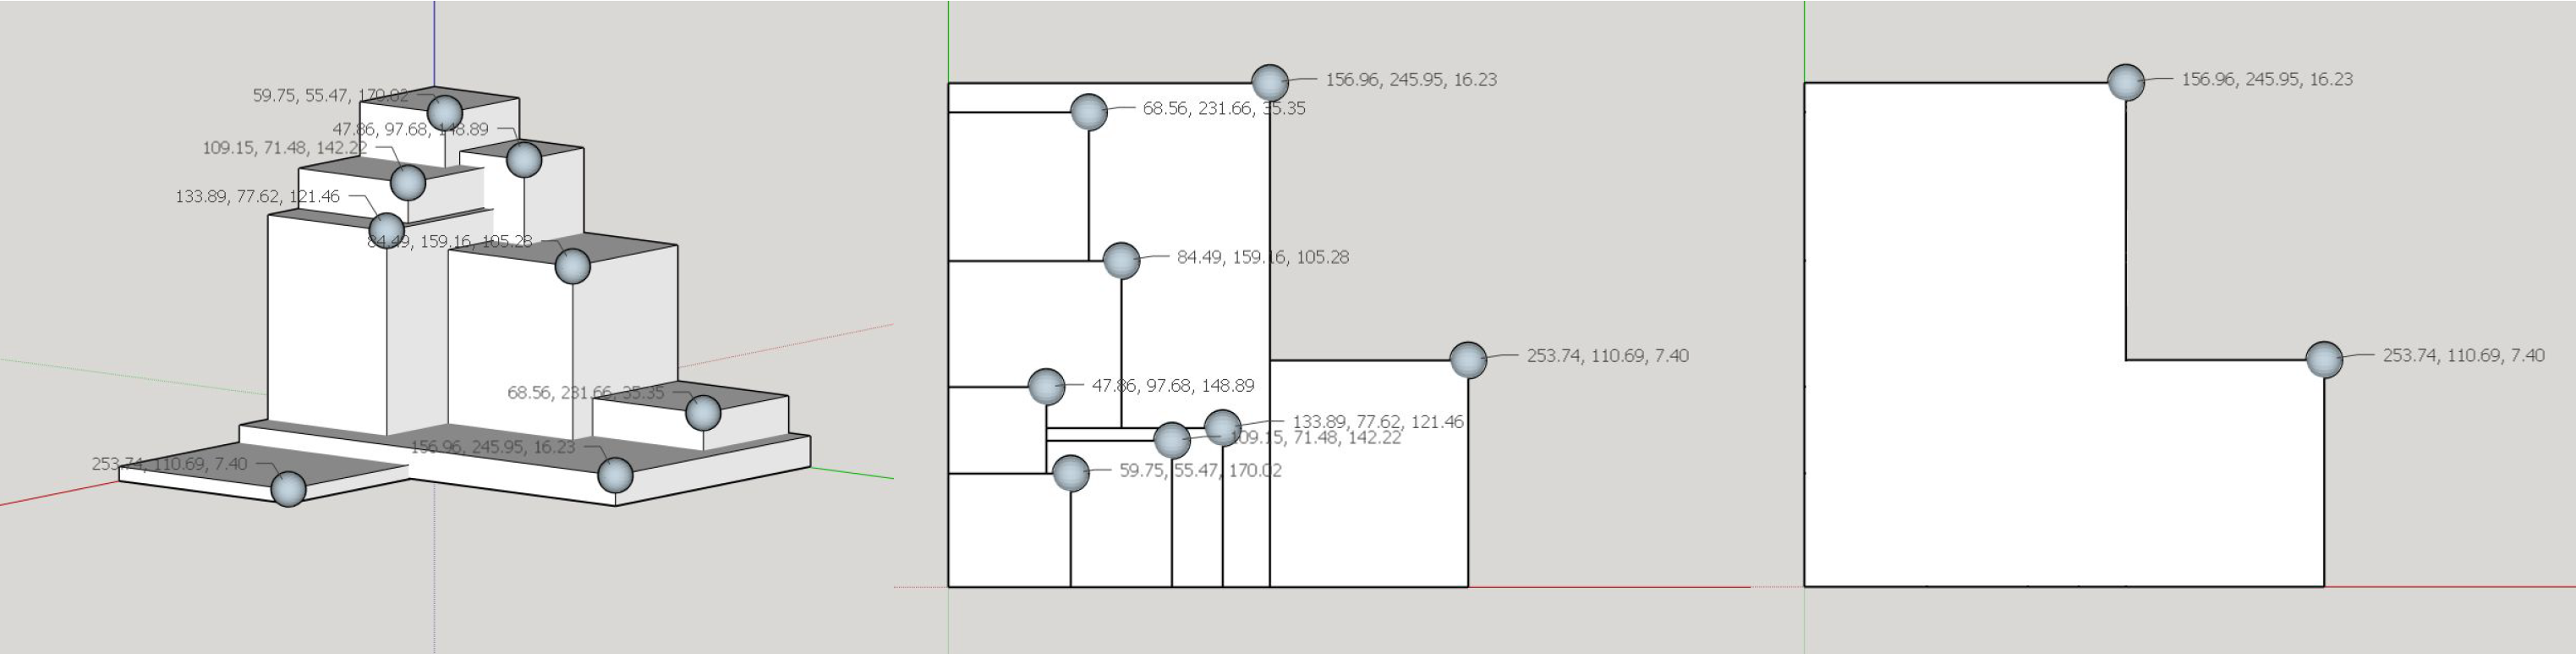
\includegraphics[width=\textwidth]{../images/CrossSection2D}
\caption[Area of 2D frontier projection]{Comparing conflict between objectives based on the area bounded by two-dimensional frontier projection. Left is the original frontier; middle shows the 2D projection of the frontier; right shows the projected frontier with all dominated solutions removed. Assuming both objectives are maximized, the larger the area bounded by the cross-sectional area, the less conflict between the objectives.}
\label{fig:frontierCrossSection}
\end{figure}